\chapter{Results}
\label{ch:results}

\section{Example units and their conditional place firing}
\label{sec:example_units}

To get an intuition of place cell activity in different experimental conditions below I provide a series of examples of single cells. This is a qualitative, not quantitative visual analysis to get an overview of the types of place fields and their spatial preference in current experimental conditions. Quantitative analysis follows in subsequent sections.

In all 3 experimental conditions of a shift experiment (see introducing mismatch between stable reference frames) I recorded putative pyramidal cells from the hippocampal CA1 region from 9 animals; 521 of these cells were classified as spatially selective (see identification of single units). As some cells had multiple place fields, for the purpose of this study I’m going to focus on individual place fields instead of single cells as more relevant for the data analysis.

\subsection{Visually-driven place cells (VPCs)}

A total number of 176 place fields showed preference for the visual reference frame. Below we provide examples of a single unit firing, selective for particular features of the visual virtual scene, like:
\begin{itemize}
  \item a dark compartment of the scene (Figure 10a)
  \item an initially invisible part of the scene (Figure 10b)
  \item virtual pillars located in the middle of two compartments (Figure 10c)
  \item several virtual boundaries (Figure 10d)
\end{itemize}

\begin{figure}
\captionsetup{format=plain}
\makebox[\textwidth]{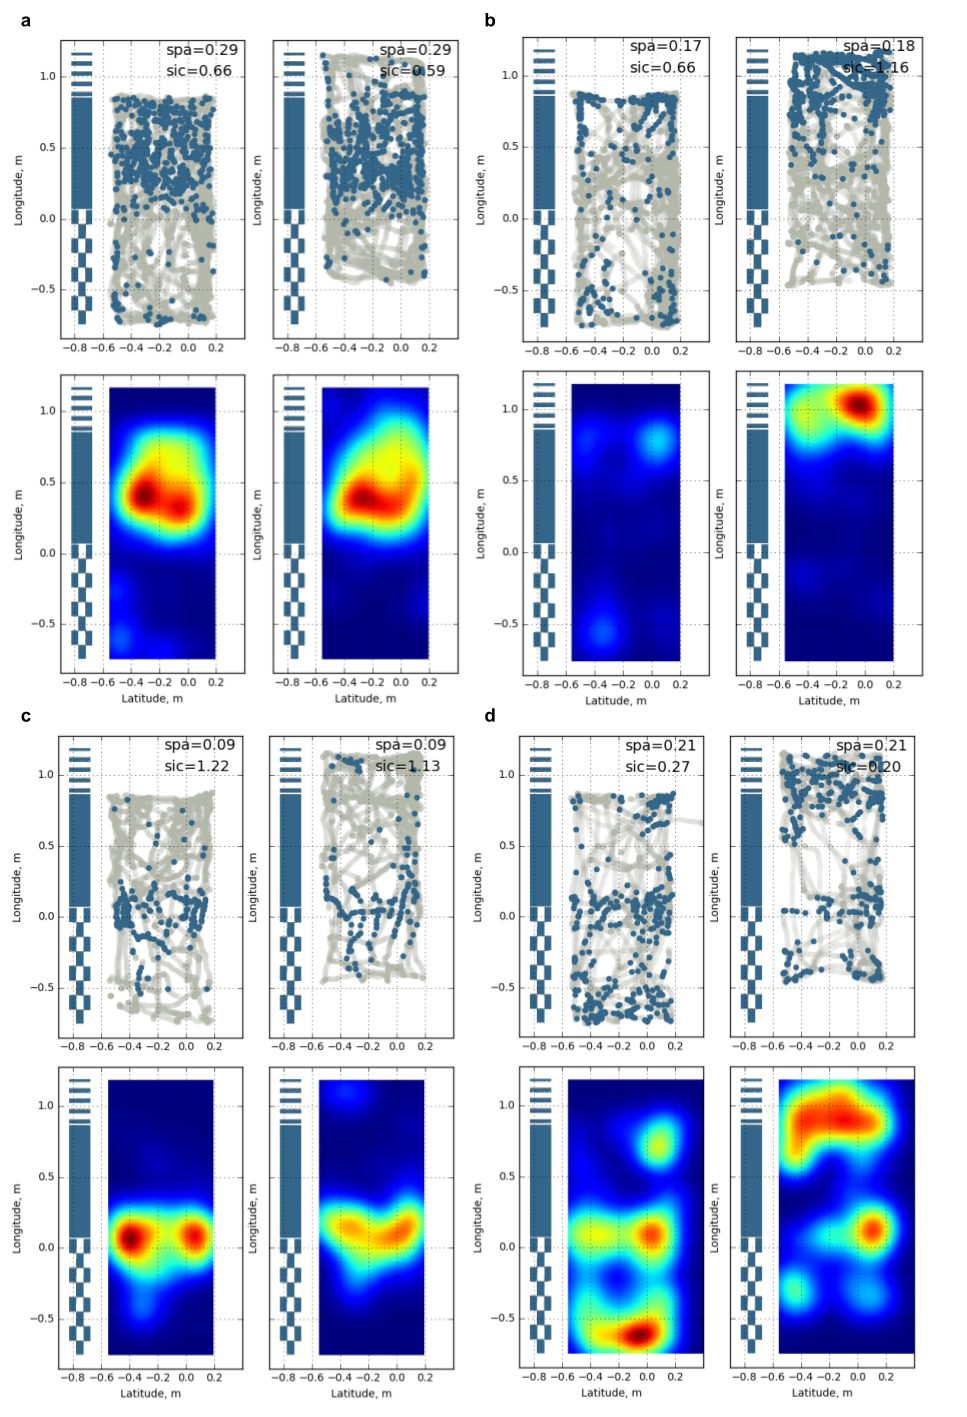
\includegraphics[width=100mm]{figures/F10_VPCs.png}}
\caption[Visually-driven place cells]{
Examples of visually-driven place cells. Each plot shows spiking (top) and firing rate maps (bottom) of a single neuron in the original and shifted arena positions. A ruler bar on the left shows schematic representation of the compartments of the (stable) virtual environment. \textbf{(a)} Cell selective for a dark compartment of the virtual environment. \textbf{(b)} Cell showing firing preference only for the initially invisible compartment, available only in the shifted position. \textbf{(c)} Cell selective for the virtual bars that make a virtual boundary inside the arena. \textbf{(d)} Cell showing preference to be active near physical and virtual borders.
}
\label{fig:F10_VPCs}
\end{figure}


\subsection{Self-motion or boundary-driven place cells (MPCs)}

A significant fraction (n=213, 29\%) of the recorded place fields showed preference for the arena reference frame. The Figure 11 demonstrates examples of the single units and their fields selective for physical arena boundaries:
\begin{itemize}
  \item for a particular corner of the arena
  \item for a particular arena boundary
\end{itemize}

\begin{figure}
\captionsetup{format=plain}
\makebox[\textwidth]{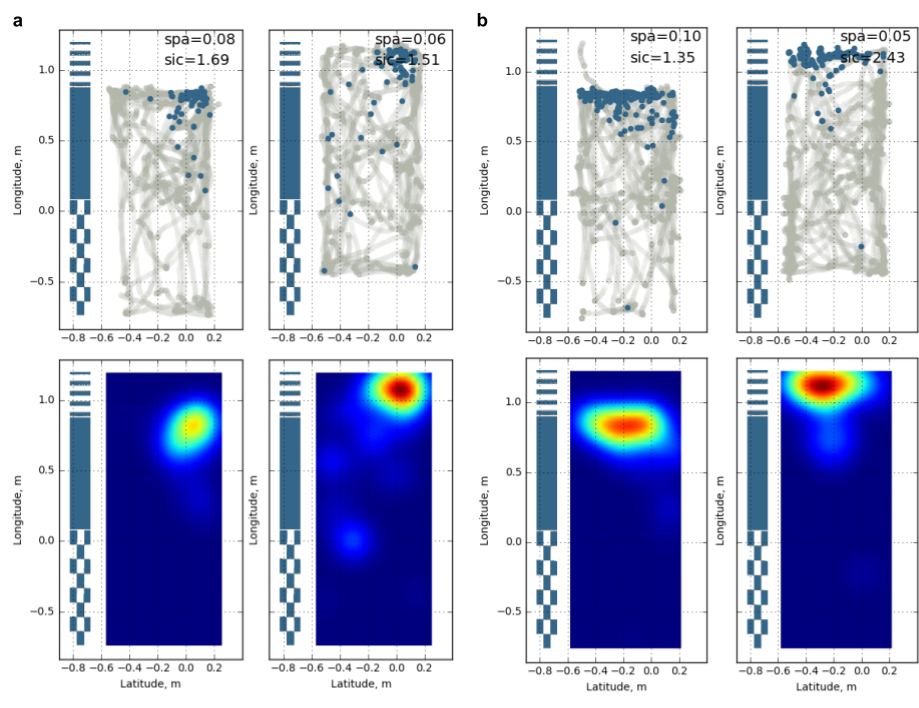
\includegraphics[width=100mm]{figures/F11_MPCs.png}}
\caption[Self-motion or boundary-driven place cells]{
Examples of boundary-driven place cells (2 cells). Each plot shows spiking (top) and firing rate maps (bottom) of a single neuron in the original and shifted arena positions. A ruler bar on the left shows schematic representation of the compartments of the (stable) virtual environment. (a) Cell active in a particular corner of the physical arena only. (b) Place cell showing preference for the upper arena boundary.
}
\label{fig:F11_MPCs}
\end{figure}


\subsection{Multi-field place cells}

On the Figure 12 I provide a couple of example cells that have multiple place fields.

\begin{figure}
\captionsetup{format=plain}
\makebox[\textwidth]{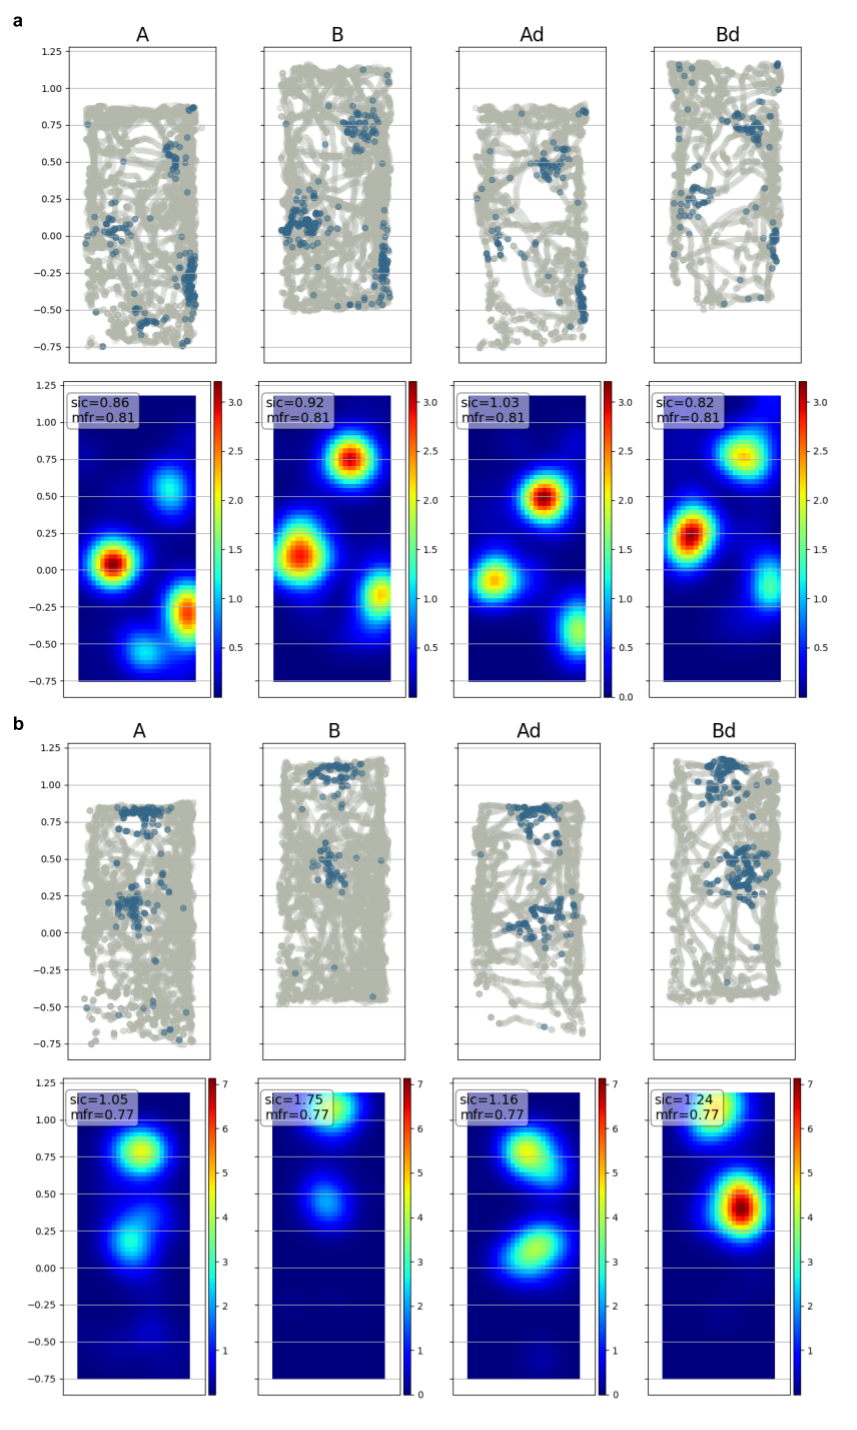
\includegraphics[width=150mm]{figures/F12_multi_field_cells.png}}
\caption[Multi-field place cells]{
Examples of multi-field place cells (2 cells). Each plot shows the schematic of the experiment (top), spiking (middle) and firing rate maps (bottom) of a single neuron in the original and shifted arena positions in light (A - B) and dark (Ad - Bd) respectively. (a) Example cell having three stable place fields. (b) Example cell having 2 fields locked to the arena reference frame.
}
\label{fig:F12_multi_field_cells}
\end{figure}


\subsection{Place cells integrating visual and self-motion components}

Recordings in conflicting sensory conditions revealed a non-bimodal distribution of place selectivity relative to the idiothetic and allocentric inputs. Many of the cells show weighted integration of both information pathways, encoding an average position. On Figure 13 is an example cell recorded in light and dark, original and shifted conditions. Note, the place field shift in light (left two columns) shows encoding of the average position defined by visual and boundary defined reference frames, while the shift gets bigger when the visual influence is lost (right column), illustrating integration of both information pathways.

\begin{figure}
\captionsetup{format=plain}
\makebox[\textwidth]{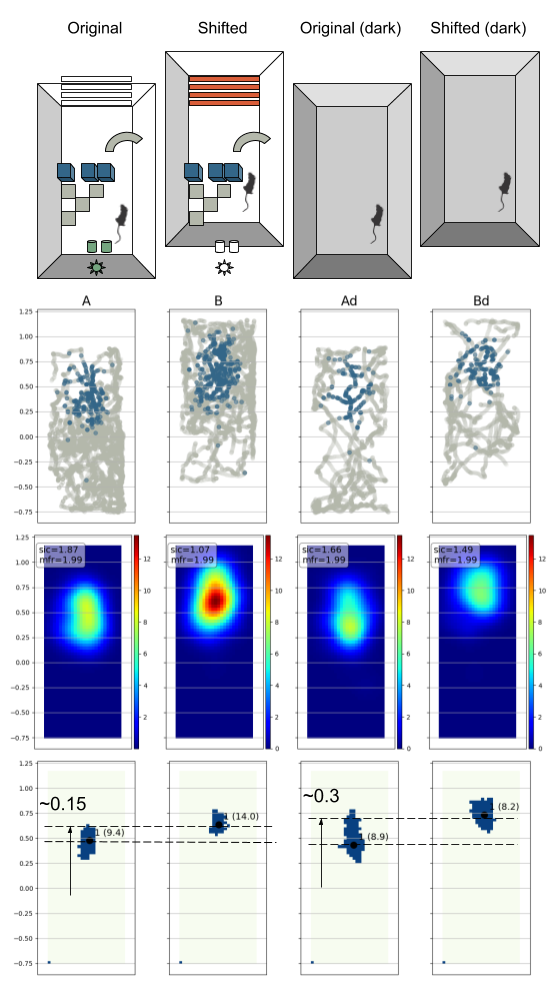
\includegraphics[width=100mm]{figures/F13_multisensory_cells.png}}
\caption[Multisensory Cells]{
Example of a multisensory place cell. Each plot shows the schematic of the experiment (top), cell spiking (second row), firing rate maps (third row) and place fields (bottom) of a single neuron in the original and shifted arena positions for light (left two columns) and dark (right two columns) positions. Dashed lines on bottom plots indicate the difference in place field shift between light and dark periods, indicating an influence of the visual information on spatial selectivity. Stability in dark shows integration of the self-motion inputs.
}
\label{fig:F13_multisensory_cells}
\end{figure}


\subsection{Multi-modal place cells}

A small portion (n=44, 6\%) of the recorded units is particularly interesting because these cells demonstrate two different types of place fields in both conditions, one encoding a particular visual landmark and another being selective for arena boundaries. Cells of this type can be identified by having one field stable between arena shifts, while the other field shifting together with the arena. These examples demonstrate an ability of a particular unit to simultaneously encode two reference frames of different type - visual and boundary-driven.

\begin{figure}
\captionsetup{format=plain}
\makebox[\textwidth]{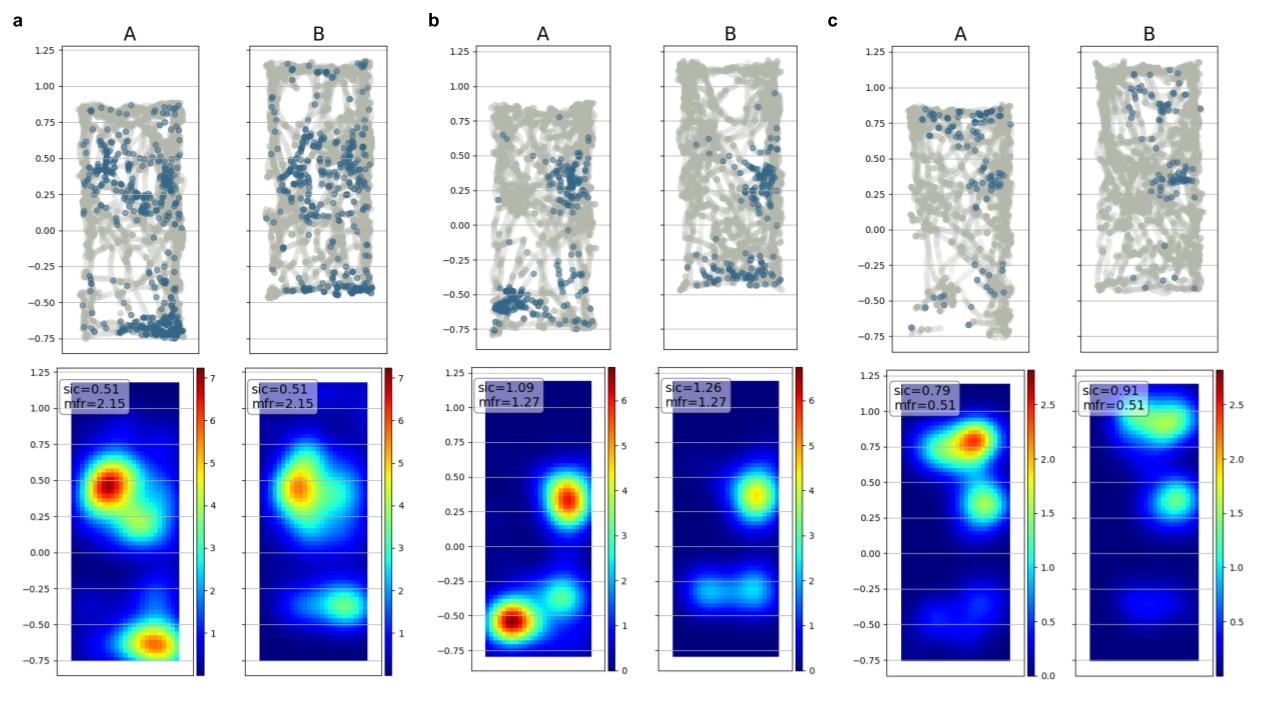
\includegraphics[width=150mm]{figures/F14_multi_modal_cells.png}}
\caption[Multimodal place cells]{
Examples of multisensory cells simultaneously encoding two reference frames. Each plot shows the schematic of the experiment (top), neuron spiking (middle) and firing rate maps of a single neuron in the original and shifted arena positions. (a) Place cell selective for the dark virtual compartment and the lower arena boundary. (b) Cell showing firing preference for the lower arena boundary and some location in the middle of the virtual environment. (c) Place cell selective for the upper arena boundary and also for some virtual location.
}
\label{fig:F14_multi_modal_cells}
\end{figure}


\subsection{Place cells expressing selectivity to specific virtual landmarks and visual features}

Several recorded units exposed specific place or domain selectivity. Figure 15 illustrates cells selective for both physical and virtual boundaries, or a cell selective for any place except a dark compartment of a virtual reference frame. These high-level encoding cells were mostly unique and cannot be statistically classified to a particular category.

\begin{figure}
\captionsetup{format=plain}
\makebox[\textwidth]{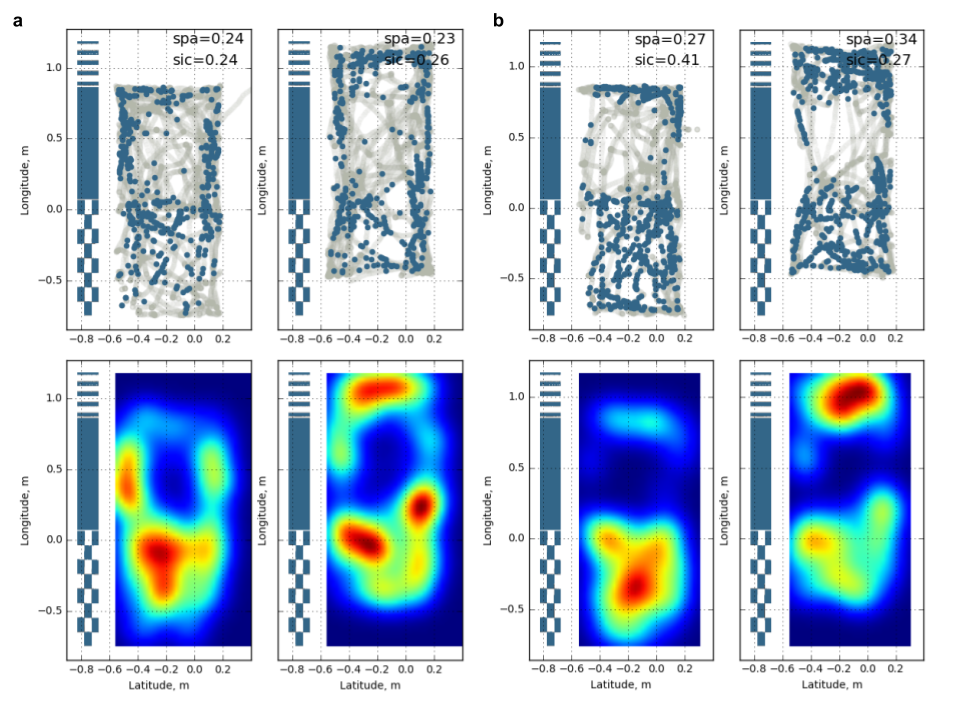
\includegraphics[width=100mm]{figures/F15_specific_cells.png}}
\caption[Specific place cells]{
Example units showing selectivity to specific virtual landmarks and visual features. Each plot shows firing rate maps of a single neuron in the original and shifted arena positions. (a) Cell representing a mixture of physical and virtual boundaries. Spiking activity near the middle of the arena corresponds to the virtual bars that make a virtual boundary. (b) Cell selective for any place in the virtual environment except a dark compartment.
}
\label{fig:F15_specific_cells}
\end{figure}


\section{Place representation is based on enclosure geometry and proximal visual landmarks in VR arena}
\label{sec:env_geometry}

First, to establish a baseline of the behavior of the place cells and their navigational map in the non-conflicting allothetic and idiothetic conditions in the ratCAVE arena, I conducted the shift experiment with a coherently moving arena and the virtual scene (see vSHIFT - coherent). In this experiment, we expect CA1 cells to encode local visual cues and arena boundaries, ignoring global room coordinates. In fact, position in the global coordinates could only be derived from either the only visible cue in the experimental room - the mirror on the ceiling, or from the vestibular stimulation, coming from the moving arena, carrying a feeling of being passively moved. We assume that neither of the two options should be applicable as the mirror is located far from the animal and is almost not visible, as well as it’s been reported that animals hardly able to update their absolute position during passive shifts (\cite{Mittelstaedt1980}; \cite{Etienne1988}).

In total 119 spatially selective cells from 4 animals (see spatial firing maps and place field detection) were recorded and then analysed using the shift detection procedure (see place field shift detection). The shift detection procedure returns the position of each place field in the two different conditions - original and shifted. For this coherent translation case, if a particular place field has a shift between original and shifted conditions similar to the translation of the arena, this would indicate the field is moving “together” with the arena (and VR scene in this coherent case) and is locked to the non-conflicting arena/VR reference frame. Conversely, if the field has no shift between conditions that would display either its preference towards some globally positioned landmark, or its ability to compute  position estimation in global coordinates based on vestibular inputs.

The mean of the resulting place field distribution appeared at the shift of 0.28m in the global (room) reference frame given arena translation of 0.3m (see Figure 16). The absence of any distribution bias towards zero shows general preference for all place cells to encode arena / virtual scene reference frames, as expected. Although from these data one cannot make a full statement, one can assure that the total majority of hippocampal place cells in these conditions ignore any external stimuli (distal cues or vestibular inputs associated with arena displacement), encoding position inside the arena based on the arena boundaries and projected visual cues only. This allows to ignore any influence of these factors for future experiments. In the meanwhile, the statistics of these sessions (mean, SD) could be very practical for the subsequent analysis to quantitatively characterize the place field shift detection method for the recorded place field data.

\begin{figure}
\captionsetup{format=plain}
\makebox[\textwidth]{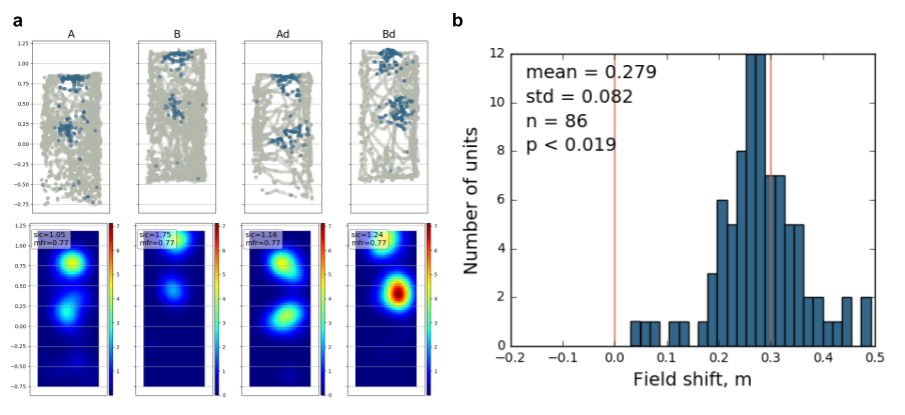
\includegraphics[width=150mm]{figures/F16_proximal_cues_geometry.png}}
\caption[Spatial orientation relative to proximal cues]{
Passive coherent movement of the whole environment (arena + visual projection) does not affect place fields firing. (a) example place cell with 2 place fields. (b) The distribution of the place fields shift between original (A) and shifted (B) conditions is centered near the actual shift of the whole environment, indicating spatial encoding based on the proximal visual cues and arena boundaries. A fraction of outliers might be due to mismatches in the shift detection procedure related with occasional low arena occupancy resulting in inaccurate place field centers.
}
\label{fig:F16_proximal_cues_geometry}
\end{figure}


\section{Place field stability in darkness can be attributed to integration of self-motion inputs}
\label{sec:integration_of_sm_imputs}

Assuming animals can only use local boundaries and projected virtual visual cues for self-localisation in the VR arena (see previous chapter), the only possibility to encode position in absence of visual cues (darkness) is to rely on integration of self-motion (path integration). If a particular place cell continues to fire in the same location in darkness indicates that it is driven either purely by self-motion, or by a combination of vision and self-motion when visual inputs are available (exceptions might be the place fields in the corners of the arena or in places where animal had left its feces, where the tactile or olfactory cues alone could define the absolute position within the arena). By quantifying the amount of place cells that keep their location preference between light and dark conditions one can build an assumption on how much of the self-motion component is integrated by the place cells in the non-conflicting (vision versus boundaries) sensory situation.

Using the field matching procedure (see place field shift detection), we split detected place fields (if a place field in original condition $F_a$ that has a pair in shifted condition $F_b$ it is one detected field F) into four categories. If a field $F_a$ has a corresponding field $F_a^{dark}$ in darkness, as well as its corresponding field $F_b$ has a pair $F_b^{dark}$ in darkness we classify this field as “stable”. If we cannot detect a corresponding pair field in dark condition for either $F_a$ or $F_b$, we classify this as “B-stable” or “A-stable” field, respectively. If neither of the fields $F_a$ or $F_b$ have a corresponding pair after the lights were turned off we classify this field F as “remapping”. The example on Figure 17 a) is a place cell with two “stable” fields.

\begin{figure}
\captionsetup{format=plain}
\makebox[\textwidth]{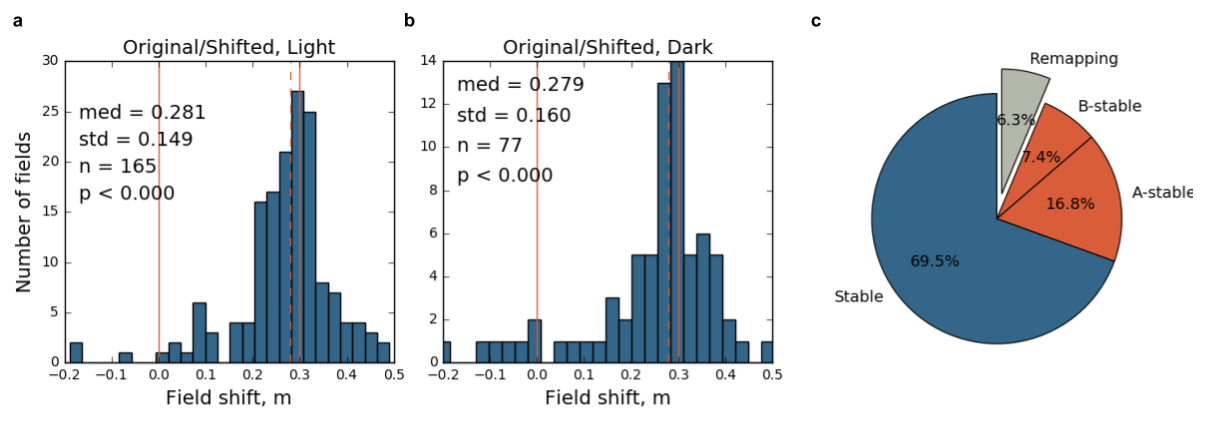
\includegraphics[width=150mm]{figures/F17_integration_of_sm_inputs.png}}
\caption[Widespread integration of self-motion inputs]{
The majority of place cells integrate self-motion inputs. Distribution of place field shifts in darkness (b) is similar to the light periods (a) in non-conflicting sensory conditions. (c) Fractions of place fields that can be tracked between light and dark periods. Only a small percentage of place fields (6.3\%) experience full remapping in darkness, indicating a high probability of integration of self-motion component for single cells, in line with previous reports (\cite{Allen6245}).
}
\label{fig:F17_integration_of_sm_inputs}
\end{figure}

A small percentage of place fields (6.3\%) experience full remapping in darkness, which could be attributed to the impaired path integration (\cite{Allen6245}). The relatively large (7.4 + 16.8 = 24.2\%) percentage of A- or B- only stable cells might be due to the decreased occupancy in the darkness condition (less running time, 4 versus 8 minutes in light) which led to the reduced quality in identification of place fields and false negatives in detection of place fields. Overall, the total domination of stable or partially-stable place fields between light and dark conditions (93.7\%) indicate that the majority of the place cells integrate position estimates based on self-motion inputs given non-conflicting sensory conditions (Figure 17c) and are not affected by the displacement of the arena with respect to the room coordinate system and are not controlled by the room-bound landmarks (mirror, projector, cameras etc).


\section{Simultaneous encoding of different reference frames}
\label{sec:integration_of_sm_imputs}

To investigate place cell behavior relative to the allocentric and idiothetic inputs we introduced a conflict between visually-defined and boundary-defined reference frames while an animal was randomly foraging inside the arena. A fraction (55\%) from the total recorded neurons (n = 521) in the vSHIFT-physical experiment demonstrate preference to either boundary-defined or visually-defined (examples in the section above) reference frame (see Figure 18a). This separation of place encoding in categories goes in line with already reported data (\cite{Mcnaughton1996}; \cite{Aronov2014}; \cite{Chen2013}; \cite{Haas2019}), however so far it’s been only shown for the cases of animal running on real track bound by reward-containing start/stop boxes or virtual linear tracks with VR-space contingent reward where it could be influenced by the reward bias. In contrast, here animals are freely-foraging  2D arena  for randomly scattered reward. Surprisingly, we found a significant number of cells (n=44, 6\%) having multiple place fields where each field was encoding a different reference frame (see Units encoding multiple reference frames). The ability of single hippocampal cells to simultaneously encode different categories of the same type of information (e.g. distal and proximal visual cues) was already presented (\cite{Knierim2002}), however this does not account for distinct types of information - visual and non-visual (self-motion or direct tactile and olfactory), presented in the current experiment. This suggests that hippocampal cells might pre-synaptically combine distinct types of sensory afferents and can be equally engaged in encoding different sensory modalities.

\begin{figure}
\captionsetup{format=plain}
\makebox[\textwidth]{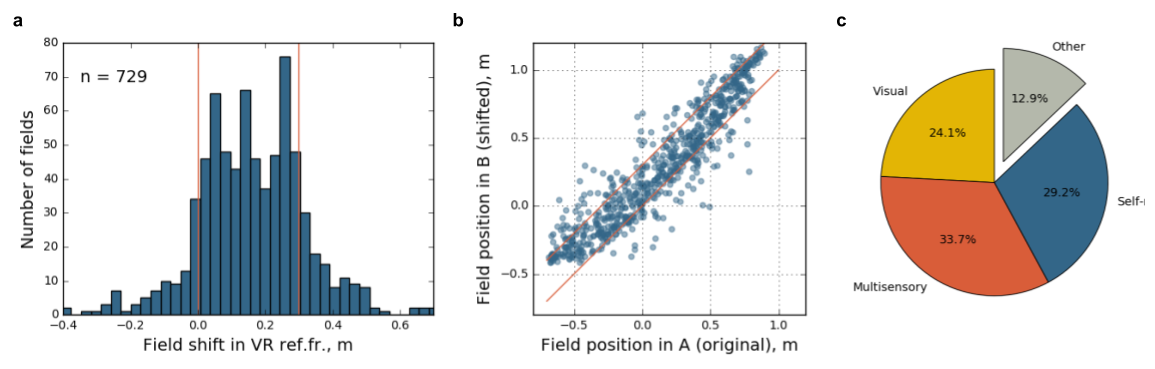
\includegraphics[width=150mm]{figures/F18_shift_distribution.png}}
\caption[Place field shift distribution in conflict]{
Place field shift enables classification of the CA1 cells into categories depending on their inputs. (a) Distribution of place field shifts between original (A) and shifted (B) conditions in the VR reference frame. Peak near zero denotes a group of place fields locked to the visual reference frame. Another peak near 0.3m defines fields encoding stable locations relative to the arena reference frame. A peak in the middle shows non-bimodal distribution of spatial selectivity in favor of a weighted integration of sensory inputs. (b) The same distribution as in (a) plotted against the position of the field in the arena in original (A) and shifted (B) conditions. Note the higher concentration of the 0.3 values near arena boundaries (bottom left and top right). (c) Overall classification of all place fields into 4 categories by their shift in conflicting sensory conditions.
}
\label{fig:F18_shift_distribution}
\end{figure}

Using the same shift detection procedure (see methods), the shifts in global (=VR) coordinates of a total of n=729 place fields from 6 animals were obtained from the recorded neural data (see Electrophysiology). The resulting place field shift distribution demonstrates place preference relative to the visual or boundary reference frames along the longitudinal axis, as well as the distribution of place fields along the arena (see Figure 18a). The distribution of place field shifts has 3 peaks around 0, 0.15 and 0.3 meters. On one hand, a non-uniformity of the resulting distribution suggests categorical structure of the underlying firing fields and corresponding neuronal mechanisms. On the other hand, a presence of the large group of place fields (n=246, 33\%) encoding average between reference frames suggests possible continuous weighted integration of visual and self-motion sensory components (see discussion about weighted integration).
A light domination of the boundary-driven over the visual place representation preference (29\% versus 24\%, cells attributed to each group by having a place field shift of 0.3m (+- ~1 SD = 0.075m) or 0.0m (+- ~1 SD = 0.075m)) can be explained by the initial larger influence of the boundaries while initially exploring the environment (\cite{Keinath2018}). Another reason can be that the recordings were made from mainly distal, not proximal CA1, which is known to get more input from the mEC representing idiothetic inputs, rather than lEC, better known to provide allothetic sensory information (\cite{Knierim2014}).

According to our analysis, a place field shift near 0 m defines a group of place fields, stable relative to the landmarks in the virtual scene during physical arena displacement (24\% cells). This allocentric stability in virtual space could be explained by a profound drive of the hippocampal cells by visual inputs. This type of neurons having fields mainly driven by vision was already established (\cite{Muller1987}; \cite{Chen2013}, \cite{Haas2019}). Another possibility would be that this group of cells receives both visual and self-motion inputs, but the self-motion component is weak and is fully reset by visual landmarks every time the animal appears to be navigating near virtual cues away from the borders. The appropriate evidence for that hypothesis still needs to be found and it is being discussed later in the following chapters.

A place field shift near 0.3 m includes a number of place fields that move together with the boundary-defined reference frame. A presence of this type of location encoding can be explained if either cells would be driven by self-motion inputs away from arena boundaries (the idiothetic path integrator, trajectory integration relative to the arena walls) or by a direct tactile contact with borders (e.g. inputs from border cells).

Similar results of separating groups of place fields into visually- and boundary-driven categories was reported in several studies (\cite{Chen2013}, \cite{Haas2019}). However a third category of place fields, representing an average location between visual-landmark- and boundary-defined reference frames, was not yet explicitly found and investigated.

To test if this category of place fields appeared by chance the random simulation procedure as there would be only two visual- and boundary- cell categories was performed. Assuming there is no average position encoding, the overall distribution of the field shifts could be represented by a sum of two gaussian distributions (visual and boundary categories) with means of 0, 0.28 and SD of 0.82 (values taken from the original vSHIFT - coherent experiment) having sample proportions as the ratio of the actual peaks around these means (1:1.2). The random simulation of such a sum of distributions reveals a 0.00001 chance of 0.33\% of all samples (246 out of 634 fields) falling between 0.075 and 0.225 (middle shift range). This is a strong evidence that this category is not a result of a chance coming from experimental recordings.


\section{Balance in availability of a certain sensory modality determines position encoding at the population level}
\label{sec:balance_sm_vs_vision}

According to the previous reports (\cite{Mcnaughton1996}; \cite{Gothard2001}) and subsequent reviews (\cite{Maaswinkel1999}) it is hypothesised that in conditions, where different spatial reference frames are in conflict with each other the place code shows a hierarchy of preferences (\cite{Maaswinkel1999}). In particular, in absence of immediate boundaries or away from the boundaries visual cues can take over. In the vSHIFT-physical experiment, the distribution of the place field shifts reveals the higher concentration of the visually-driven fields in the center of the arena (e.g. away from the northern and southern arena boundaries), while having a higher concentration of boundary- or self-motion driven fields near the borders (see Figure 19a, b). This could be explained by a competition of boundary-driven self-motion and visual inputs. Close to the environmental boundaries the direct tactile contact engages additional sensory modalities, while the quality of visual projection decreases. Away from the boundaries all the visual cues are instantly available while the precision of the self-motion based inputs decays with time and distance travelled since the last boundary, although not that fast to be very distorted in current experimental conditions (\cite{Hardcastle2015}). This allows to hypothesize, that if a place cell encodes a combination of the self-motion and visual components, the contribution of the visual one would be larger in the center of the arena, setting a higher weight for that type of an input. Opposite, near the boundaries the contribution of tactile / self-motion component would overtake the vision and a place field input weights would be more balanced towards self-motion. More of the interpretation of these findings in the discussion.

\begin{figure}
\captionsetup{format=plain}
\makebox[\textwidth]{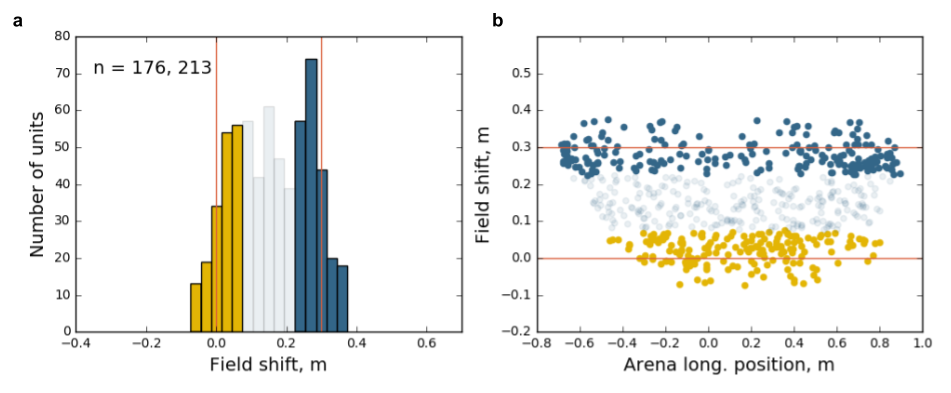
\includegraphics[width=150mm]{figures/F19_balance_field_concentration.png}}
\caption[Balance between vision and self-motion]{
Balance in concentration of fields of different types (vision versus self-motion) in the center versus near the boundaries of the arena demonstrates a tendency to prefer more available sensory input for spatial encoding, potentially implementing optimal coding at the population level. (a) Distribution of place field shifts between original (A) and shifted (B) conditions with visual (yellow) and self-motion (blue) groups highlighted. (b) Place field shift plotted against position in the arena. Visual and self-motion groups highlighted as in (a).
}
\label{fig:F19_balance_field_concentration}
\end{figure}


\section{Removal of allocentric information reveals a group of multisensory CA1 cells to be driven by a combination of vision and self-motion}
\label{sec:multisensory_integration}

To further investigate the interaction of the hippocampal place cell afferents, we recorded several sessions of the original vSHIFT-physical experiment having a darkness period after the main session time. This allowed to analyse the change in spatial selectivity for place fields, especially the fields driven by a combination of visual- and self-motion inputs, when the visual input together with the whole virtual reference frame are absent. Essentially by looking at the change in cell activity - change in firing rate, field size, field shift or complete re-mapping - we can hypothesize how the reduction of sensory input, in particular, visual information influences place cell binding to a specific reference frame.

For the light periods, place field shift distribution for sessions with darkness is equivalent to the regular shift experiment sessions (see Figure 20a). However, taking the darkness periods alone, all identified place field shifts are centered around 0.28m with no substantial amount of fields near 0.0m, showing their preference to encode the boundary-defined reference frame (Figure 20b). Intuitively, this is logical: the only way to encode the position in the global (or visual, when the projection is on) reference frame in darkness is to integrate the vestibular information about the arena translation and keep this information intact in relation to the arena borders. This would be unexpected, first, because the information about the passive move is normally not used by the animal to represent the local environment (see the results from vSHIFT - coherent), and second, because there is no clear evidence that path integrator can ever maintain absolute positional information during passive translations based on the vestibular inputs only.

Likewise, the distribution of the place field shifts along the arena in light shows equivalence to the regular experimental sessions, having higher concentration of the visually-driven (shift 0.0m) place fields in the middle of the environment and higher concentration of the boundary-driven fields (shift 0.3m) near the boundaries. The distribution of the fields in darkness confirms absence of visually-driven cells, and additionally displays higher shift variance (not shown) for fields in the middle of the arena, pointing to a reduced precision of position encoding. As most of the cells in dark are driven by self-motion or boundary-defined cues, this could be taken as another light evidence of error accumulation by path integrator away from the reference point.

\begin{figure}
\captionsetup{format=plain}
\makebox[\textwidth]{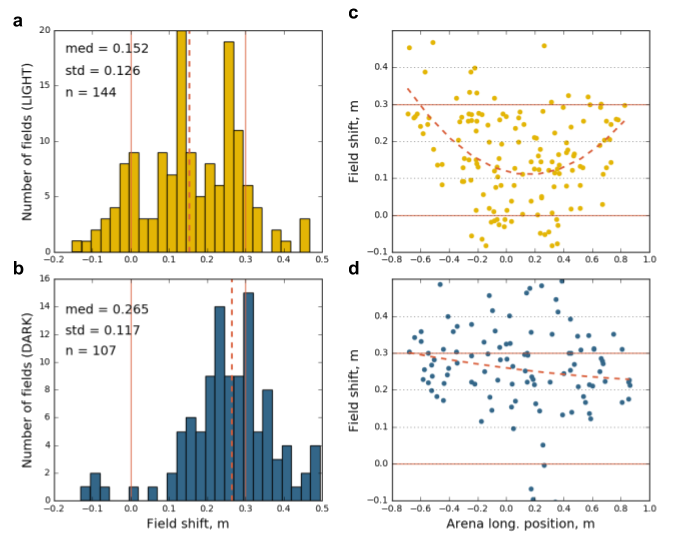
\includegraphics[width=150mm]{figures/F20_light_versus_dark.png}}
\caption[Place fields in light and in dark]{
Change in place field shift distribution for the vSHIFT-physical experiment between light and dark conditions. (a) Distribution of place field shifts in light. Similar to Figure 18a. (b) Distribution of place field shifts in the dark shows that most of the cells rely on path integration in absence of visual input (average shift near 0.3m). Distribution of the place fields of different types inside the arena in light (c) and in dark (d) confirms higher concentration of the visually-driven cells away from the arena boundaries (see next section).
}
\label{fig:F20_light_versus_dark}
\end{figure}

Overall, the dark period is characterized by the reduction in the mean firing rate (by 10\% average, t(146)=-4.38, p<.00002) and decrease in sparsity (by average 15\%, t(146)=-7.85, p<.00001). This might be explained that the loss of visual input, that decreases the overall amount of incoming excitatory activity to the hippocampal circuit, also leads to the reduction in the spiking probability of the place cells in the pyramidal layer. The overall increase in information content (by average 9\%, t(146)=5.21, p<.00001) might be explained by the increased proportion of fields near the boundaries in darkness which are in general more precise (see fine position calibration near the boundaries).

Looking at the place field maps and visually analysing changes of the field locations and place cell activity between light and dark conditions a number of typical cases show up: a) place field firing is completely abolished (see Figure 21a), place field stays in the same location with no substantial change in firing rate (see Figure 21b), place field loses spatial selectivity, changes its firing rate or remaps to a new location within the arena (see Figure 21c). For a more detailed analysis, we separate the resulting fields in 4 groups using the field matching procedure (same as for vSHIFT - coherent, see place field shift detection). If a field $F_a$ has a corresponding field $F_a^{dark}$ in dark, as well as its corresponding field $F_b$ has a pair $F_b^{dark}$ in dark we classify this field as “stable” - these fields keep firing along the whole session in corresponding light and dark periods. If we cannot detect a corresponding pair field in dark condition for either $F_a$ or $F_b$ , we classify this as “B-stable” or “A-stable” field, respectively. If neither of the fields $F_a$ or $F_b$ have a corresponding pair after the lights were turned off we classify this field F as “remapping”.

\begin{figure}
\captionsetup{format=plain}
\makebox[\textwidth]{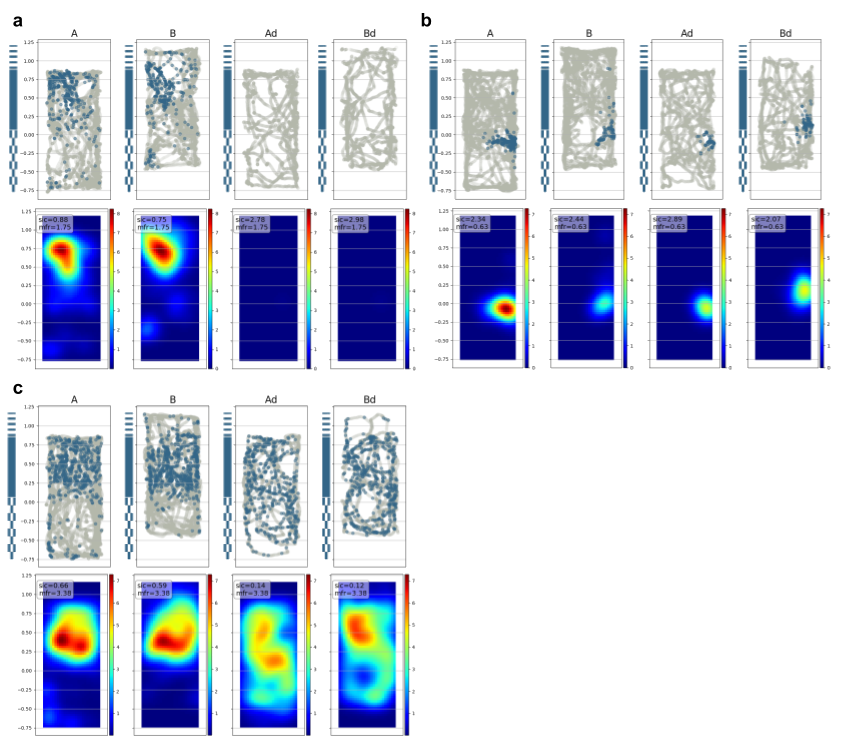
\includegraphics[width=150mm]{figures/F21_remapping_types.png}}
\caption[Remapping in darkness]{
Different types of changes in place cell behavior after the lights are off. (a) An example place cell that goes fully silent in dark. (b) An example place cell with stable location and mean firing rate between light and dark condition shows independence of the visual reference frame. (c) An example cell showing preference for a particular visual part of the environment exposes complete remapping in dark.
}
\label{fig:F21_remapping_types}
\end{figure}

A bit more than a half of the population of fields goes to the stable group (see Figure 3.11a). Their stability might be due to these cells getting strong self-motion inputs which do not reduce their sharpness (\cite{Allen2016}) and which enable them to keep their stability in darkness. The unstable group, comprising partially stable (place field can’t be detected in both original and shifted positions in dark) and fully remapped fields, react by a significant amount of change to the loss of the visual input and the virtual reference frame.  The contrast between the groups is of  particular interest for investigation relative to their shift preference, which could be attributed to the amount of allocentric and idiothetic information that drive their activity.

The place field shift distribution for the stable group contains a substantial amount of field shifts centered at 0.15 and at 0.3, which correlates with the assumption that these fields are mostly self-motion / boundary-driven and the underlying place cells receive a strong input of information from the self-motion (see Figure 22a). In contrast, all cells in unstable groups are balanced towards 0.0m shift, having field shifts centered at 0.0m and 0.15m and less around 0.3m. This distribution could be explained by assuming that many place fields, driven by visual allocentric information (field shift around 0.0m), when they lose their main driving input, remap or go unstable, thus belong to unstable groups. The correlation between the amount of self-motion input and cell firing stability can be also illustrated by the normalized difference of these field shift distributions (see Figure 22e), which shows negative peak around 0.0m (unstable fields having 0.0m field shift) and positive around 0.3m (more stable field shifts near 0.3m), putatively separating the groups to mostly allocentric- and mostly idiothetic- driven units. Besides field shifts, there is no significant change in mean firing rates for the stable but not for the unstable groups, accordingly. The reduction in mean firing rate might be explained by the loss of visual inputs.

\begin{figure}
\captionsetup{format=plain}
\makebox[\textwidth]{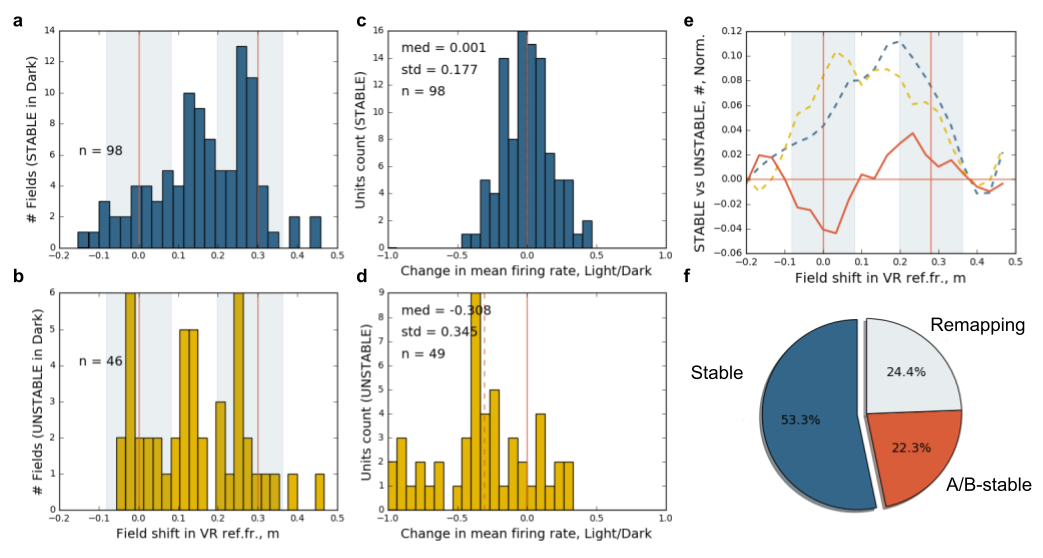
\includegraphics[width=150mm]{figures/F22_stable_unstable.png}}
\caption[Stability explained by self-motion inputs]{
The stability of the cell activity in darkness is correlated with the balance between its visual and self-motion afferents. Distribution of the place field shift (a-b) and change in mean firing rate (c-d) for the stable (cell continues to fire in darkness, top row) and unstable (cell remaps in dark, bottom row) groups. Note that significant reduction in mean firing rate for the unstable group (bottom right) suggests dependency of these cells on the visual inputs. (e) Difference between normalized distributions of place field shifts between stable and unstable groups. The plot shows more visually-driven fields (0m-shift) go to the unstable group, while more self-motion fields (0.3m-shift) go to the stable group, showing a correlation between an amount of shift in light (dependency on the visual reference frame) and firing stability in darkness. (f) Overall classification of all place fields into 3 categories by their stability between light and dark conditions.
}
\label{fig:F22_stable_unstable}
\end{figure}

More intriguing result shows up when analysing the change in place field shift distribution of the stable group between the light and dark conditions. The 0.3m boundary-driven group, assumed to be composed of units mostly driven by self-motion inputs, does not show any change in its shift preference (see Figure 23a, stars). The group of fields near 0.0m, putatively mostly driven by visual cues, loses their 0.0m shift preference and gets a high variance (not shown). Importantly, the middle “multisensory” 0.15m unit group change their shift preference from encoding an average between self-motion and visually given distances (0.15m) to an average shift of 0.3m, indicating the visual input can no longer influence the path integrator for these units and these cells stay driven by the idiothetic inputs only.

Furthermore, the detailed analysis of the place field position shifts for the multisensory 0.15m unit group reveals that in both original and shifted conditions the shift is directed towards the middle between their corresponding place field locations in dark (see Figure 23b). To be more precise, in the original arena position the place field in light is “ahead” of its corresponding field in dark (when it’s self-motion driven only), as the same time for the shifted position the field is “behind” its corresponding field in dark. This direction of the shift is unique to the multisensory group as, for instance, this is not the case for the pure self-motion driven group of cells (see Figure 23c). Altogether this points to the special type of integration of visual with self-motion information. The possible underlying mechanisms are provided in the discussion.

In summary, the change of the place cell firing in darkness confirms the different amount of visual- and self-motion inputs distributed among the 0.0m, 0.15m, and 0.3m shift groups. This suggests the continuous connection between the amount of influence of an allocentric input versus idiothetic inputs and a cell behavior in darkness, ranging from the remapping, if the cell is more visually-driven, to the stable place field in case the self-motion inputs are dominating. The substantial amount of units having 0.15m shift demonstrate the ability of the hippocampal circuitry to use weighted combination of inputs and represent places centered at the average between visual-landmark- and self-motion or boundary-defined distances.

\begin{figure}
\captionsetup{format=plain}
\makebox[\textwidth]{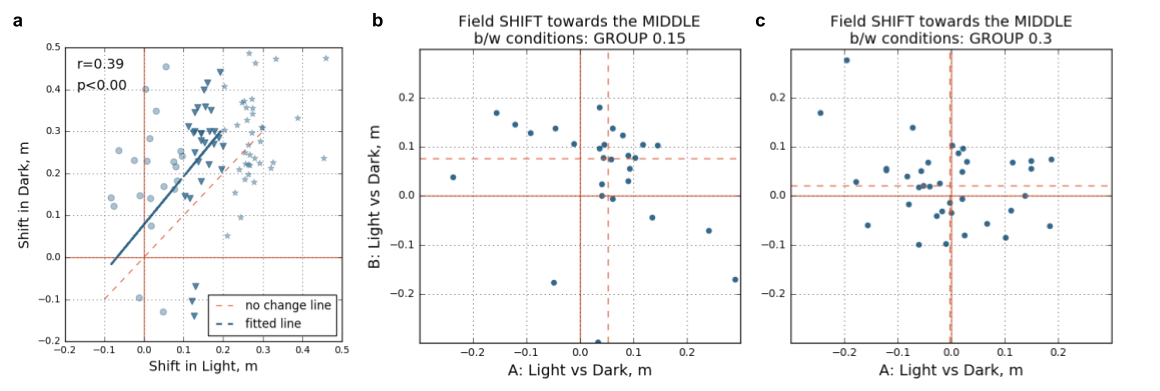
\includegraphics[width=150mm]{figures/F23_shift_to_middle.png}}
\caption[Weigthed combination of the inputs]{
A detailed analysis of place field shifts of the multisensory cells shows the integration of the visual and the self-motion components as a weighted combination. (a) For the stable group, the plot shows place field shift in light versus shift in dark. For the 0.3m fields (stars) place field shift is not different between conditions showing their independence from the visual reference frame. Note that the 0.15m group (triangles) the shift in dark grows to 0.3m showing a switch to the purely self-motion based navigation. (b) Relative shifts in the same arena positions for the 0.15m group show that visual information calibrates the spatial representation towards the middle between the reference frames. For the 0.3m group (c) relative shifts in the same arena positions are not significant probably because of visual independance (right plot).
}
\label{fig:F23_shift_to_middle}
\end{figure}


\section{Fine position calibration near the environmental boundaries}
\label{sec:fine_position_calib}

In the vSHIFT - physical experiment the distribution of place field sizes relative to their arena locations points to a more precise (smaller fields) place encoding near the arena boundaries, rather than in the center of the arena (larger fields, Figure 24a). One explanation of the observed effect might be due to the cells that are getting self-motion inputs tend to be less precise away from the boundaries due to error accumulation in the underlying path integration (\cite{Etienne1996}). Cells closer to the boundaries can easier reset their self-motion dependent component due to the wall proximity, thus being able to more precisely encode actual location. However, this could be also attributed to the increased sensory information due to the direct contact with boundaries (boundary cells). This change in field size, converted to position encoding reliability, was used in the study demonstrating bayesian inference for position encoding by the hippocampal place cells (\cite{Madl2014}).

\begin{figure}
\captionsetup{format=plain}
\makebox[\textwidth]{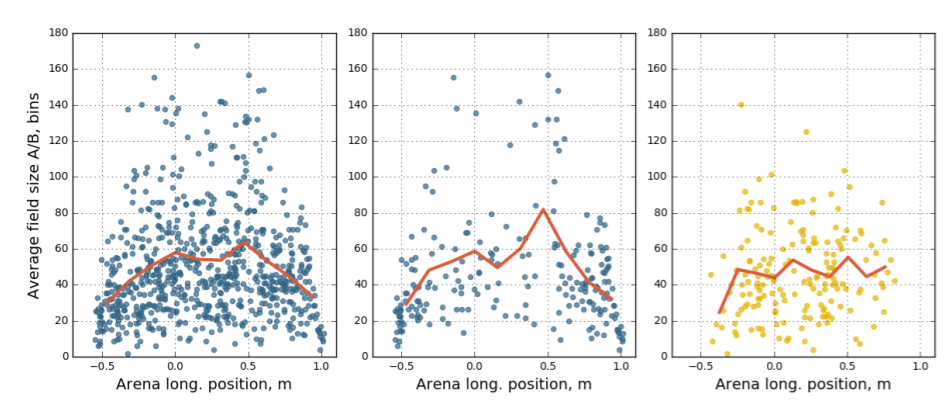
\includegraphics[width=150mm]{figures/F24_field_sizes.png}}
\caption[Position accuracy based on fields sizes]{
The distribution of place field sizes inside the arena. All place fields (left plot) and two groups of self-motion (middle) and visually (right plot) driven fields, classified as in vSHIFT -physical. Smaller sizes of place fields near the boundaries suggest higher quality of spatial orientation.
}
\label{fig:F24_field_sizes}
\end{figure}


\section{Conflict induced by physical arena translation is comparable to the translation of the visual reference frame}
\label{sec:visual_physical_equal}

In order to verify whether the information about the passive move during arena translation and the propagation of this information to the brain circuits through vestibular system is required for the successful encoding of either of the visual- or boundary- reference frames, we conducted visual shift experiment (vSHIFT - visual, Figure 25a). The protocol for the visual shift experiment was exactly matching the physical shift experiment, with the only difference that instead of the arena move for 0.3m, the visual projection was moved 0.3m keeping the same speed, such that from inside the arena the only possibility to distinguish whether the physical arena or the virtual projection is moved is to attend to the vestibular system informing about the start and the end of the passive move, or possibly to the tactile receptors informing about the vibrations during the physical arena move (Figure 25a).

In total 209 place fields were recorded in visual shift condition. Analysis of the place field shift distribution demonstrates presence of field shifts around 0.0m, 0.15m and 0.3m, showing the ability to use both visual and boundary defined reference frames for position encoding (see Figure 3.13c). High concentration of field shift in the middle of the distribution near 0.15m confirms the tendency of the hippocampal cells to encode the location centered at average between the visual and boundary defined estimates, similar to the physical arena shift condition. The comparison of the place field shift probability distributions between the physical and visual experiments (Figure 25d) demonstrates that even without the vestibular or tactile information about the passive move the visual information alone, when stable for at least 30s periods of time, can influence the positioning of the place fields and overall has very similar impact on formation of the hippocampal place code.

\begin{figure}
\captionsetup{format=plain}
\makebox[\textwidth]{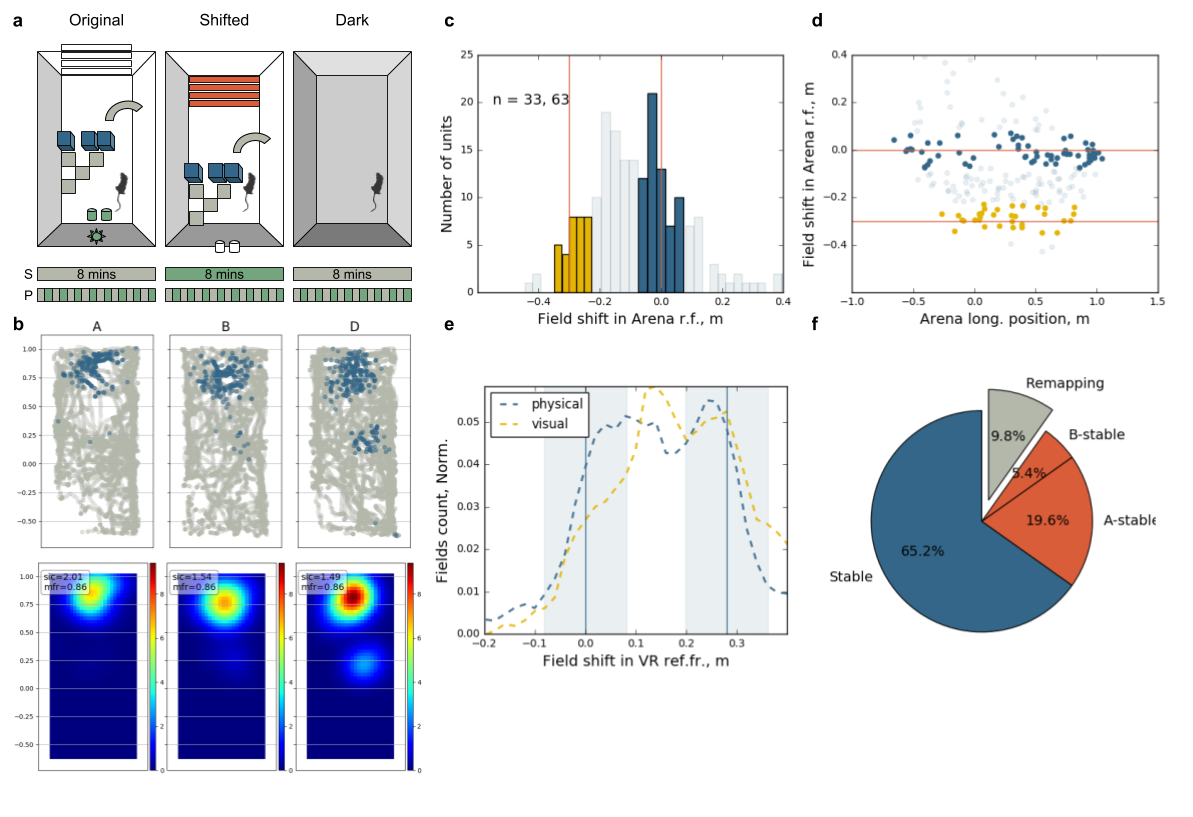
\includegraphics[width=150mm]{figures/F25_visual_equals_physical.png}}
\caption[Visual shift induces sensory conflict]{
vSHIFT-visual. (a) Schematic of the experimental protocol. (b) Example place cell spiking (top) and firing rate maps (bottom) for original, shifted and dark conditions. (c) Distribution of place field shifts is similar to the vSHIFT-physical experiment. (d) Same as in the vSHIFT-physical, there is a higher concentration of the visually-driven fields in the center of the arena, confirming the tendency to rely on the more available reference frame at the population level. (e) Comparison of normalized place field shift distributions between physical (arena moves) and visual (projection moves) types of experiments. (f) A substantial (90.2\%) amount of cells continue to be active in the dark showing widespread integration of the self-motion component.
}
\label{fig:F25_visual_equals_physical}
\end{figure}


\section{Visual conflict induces recalibration of the self-motion based place map}
\label{sec:recalibration}

Similar to the vSHIFT-physical, for several sessions in vSHIFT-visual we recorded navigation in the dark after the shifted condition. This allowed us to analyze the contribution of the induced visual mismatch to the self-motion based representation of the environment. At first, as many place cells integrate both self-motion and visual inputs, we assumed that turning the light off after “shifted” (B) condition would just cut off the visual part and bring the overall place representation into the “original” (A) learned state. In other words, for place fields that are active in dark we expect that place field would shift back to match the original position in A, because of the loss of the visual influence.

\begin{figure}
\captionsetup{format=plain}
\makebox[\textwidth]{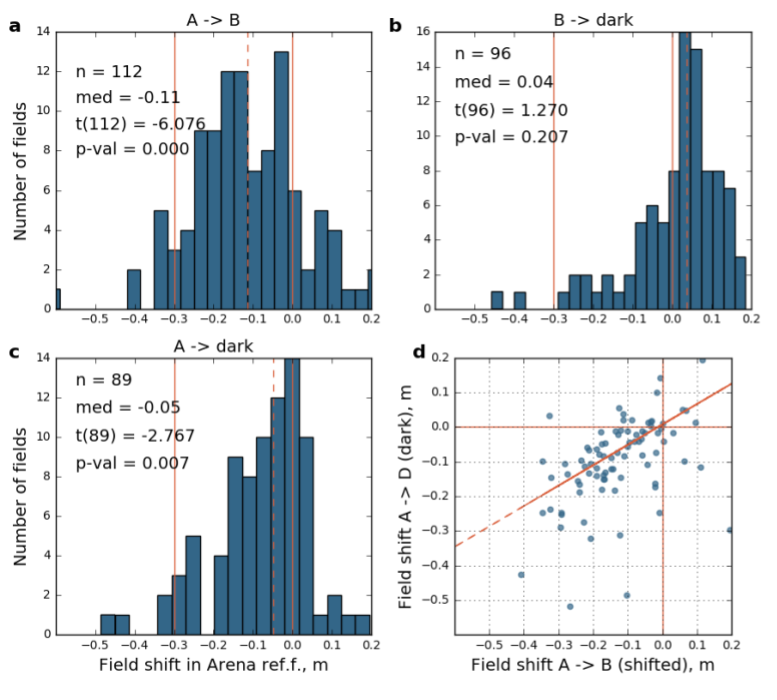
\includegraphics[width=110mm]{figures/F26_recalibration.png}}
\caption[Recalibration of the self-motion map]{
Visual conflict induces recalibration of the idiothetic self-motion based place map. (a) Distribution of the place field shift in light (A -> B) shows the influence of the conflicting visual reference frame and suggests encoding in a weighted combination manner. (b) a very little place field shift back after the lights are off (non-significant) shows that the overall spatial representation was recalibrated during conflicting condition. (c) Direct comparison of original (A) and dark (D) conditions confirms the recalibration of the spatial map as in (b). (d) A correlation between the field shift in light (e.g. its dependency on vision) and the resulting shift of the field (A -> Dark) demonstrates the connection between the amount of visual input and its influence on recalibration.
}
\label{fig:F26_recalibration}
\end{figure}

Surprisingly, this appears not to happen. As described in the previous chapter, on the population level there is indeed a place fields shift between original A and shifted B conditions (Figure 26a, n is smaller comparing to 25c as only sessions with dark periods are taken into account) due to the conflict induced by a shifted visual reference frame (by -0.11m average, t(112)=-6.07, p<.00002, Figure 26a). However, the shift “back” to the original representation is not significant (0.04m average, t(96)=1.27, p=0.2, Figure 26b). The same is confirmed by looking at the place field shift distribution between original A and dark D conditions (-0.05m average, t(89)=-2.76, p=0.007, Figure 26c). Taking individual fields and their shift induced by a visual-to-self-motion conflict versus the shift between original condition and darkness one can see, that cells that have a larger shift in conflicting conditions (more influenced by vision) tend to recalibrate more relative to their original position (Figure 26d). The interference of two reference frames led to a new state of the spatial map, where place code represents the weighted combination of them.

The results demonstrate that the self-motion based and visual landmark-based spatial representations are interconnected. Conflict induced by the shifted visual reference frame leads to recalibration of the whole spatial representation system, including the self-motion based representation. How can the change in place representation in the upstream CA1 area influence the self-motion based representation, located hypothetically in the downstream cortical areas (e.g. head-direction, speed, grid cells)? Theoretically, this recalibration could be implemented via backprojections from the hippocampal CA1 to the entorhinal system via subicular pathways. This has been already hypothesized and similar results were collected in the modelling study (\cite{Li2020}).


\section{Gradual mismatch between sensory inputs confirms weighted position estimation at smaller conflicts}
\label{sec:gain_12}

To further investigate the change in spatial selectivity of hippocampal cells in an continuously growing sensory conflict we designed an experiment with gradually increasing mismatch between position estimations coming from two different reference frames. By inducing a visual to self-motion instantaneous gain difference along the longest dimension of the arena in an asymmetric way we assume that the gain mismatch between self-motion and visual flow would affect path integration, providing a way to test its contribution to the CA1 place code, as well as allowing to test whether place fields would gradually follow the mismatch estimating position as a weighted combination of both types of sensory inputs.

\begin{figure}
\captionsetup{format=plain}
\makebox[\textwidth]{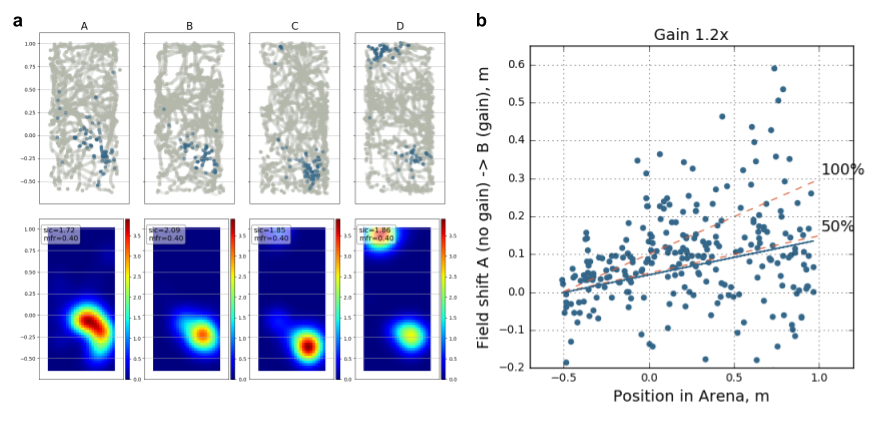
\includegraphics[width=150mm]{figures/F27_gain_12x.png}}
\caption[Sensory integration in gradual mismatch in vGAIN 1.2x]{
vGAIN 1.2x experiment. (a) An example place cell with a field active in all conditions. The gradual shift of the field along the shift of the visual reference frame (north -> south) shows influence of visual objects and cues. (b) Place field shifts between no-gain (A) and gain (B) conditions plotted against  the position in the arena. Dashed lines indicate the amount of conflict between visual and boundary-defined reference frames (100\% reflects the amount of conflict at the Y-axis). Note neurons encode the weighted average between two reference frames (blue linear regression bar), that linearly grows with the amount of conflict, on the population level.
}
\label{fig:F27_gain_12x}
\end{figure}

In the first phase (A) of the vGAIN experimental session animals were learning the stable virtual environment, coherent with environmental borders. The slow transition to the vGAIN 1.2x phase (B) introduced a visual to boundary-defined conflict in self-location ranging from no conflict near the southern arena wall to the 0.3m conflict near the northern arena wall. In line with previous vSHIFT experiments, we expect no place field shift at the southern wall followed by a gradual increase in the shift towards the northern arena wall up to a 0.3m, when comparing the initial (no-gain) and gain conditions.

In total, 275, 316 and 253 place fields from 4 animals were recorded in the vGAIN 1.2x experiment for each condition (no gain - gain - no gain shifted), respectively. An example place field, showing an influence of the conflicting visual inputs is presented in Figure 27a. Although we encounter a variance of place field shifts for different parts of the arena between no-gain and gain conditions, on the population level, we see that there is a gradual influence of the visual- to self-motion conflict along the arena, as expected. Specifically, cells tend to encode the average between the estimations given by two conflicting reference frames, positively correlated with the gradually increasing conflict (Figure 27b), providing more evidence for the hypothesis regarding the weighted combination of sensory inputs by hippocampal cells.


\section{Abandonment of a particular sensory estimate at larger sensory conflicts}
\label{sec:gain_12}

It has been shown for different sensory modalities and different animal species and also humans, that information from the internal body and environmental cues are integrated at small sensory conflicts to increase response precision (see Optimal combination of environmental cues). However, as proposed in several studies, it is reasonable to abandon less reliable sensory input in case of large conflicts  (\cite{Sjolund2018}; \cite{Cheng2007}). To test whether there is a change in place cells behaviour at larger conflicts we conducted an asymmetric vGAIN 1.4x experiment following the same vGAIN protocol, which enabled to record 1.4 gain mismatch between vision and self-motion, as well as to analyze the gradual increase of conflicting position estimation ranging from 0 to 0.6m.

Similar to the vGAIN 1.2x, the first, exploratory phase, followed by a gain condition where we induced an asymmetric 1.4x gain between self-motion and visual flow. The asymmetry enabled it to build a gradual conflict along the arena, from northern (0 conflict) to southern (0.6m conflict) wall. Taking into account an average place field size of 0.42m within these experimental conditions, the smaller gain of 1.2x and the conflict of 0.3m would still keep the incoming pre-synaptic inputs, defined by different reference frames, overlap, potentially bringing a situation to a smaller sensory conflict category, where the integration of sensory inputs makes sense. In contrast, the gain of 1.4x would build larger conflicts exceeding the average place field size, making self-motion and visual inputs completely uncorrelated in space and time. This conflicting condition might bring many place fields to the larger conflict category, where it makes sense to abandon one of the inputs. In that case, we would expect cells to prefer self-motion or path integration relative to the visual cues, as reported previously for human and rat studies (\cite{Sjolund2018}; \cite{Zhao2015}; \cite{Shettleworth2005}).

\begin{figure}
\captionsetup{format=plain}
\makebox[\textwidth]{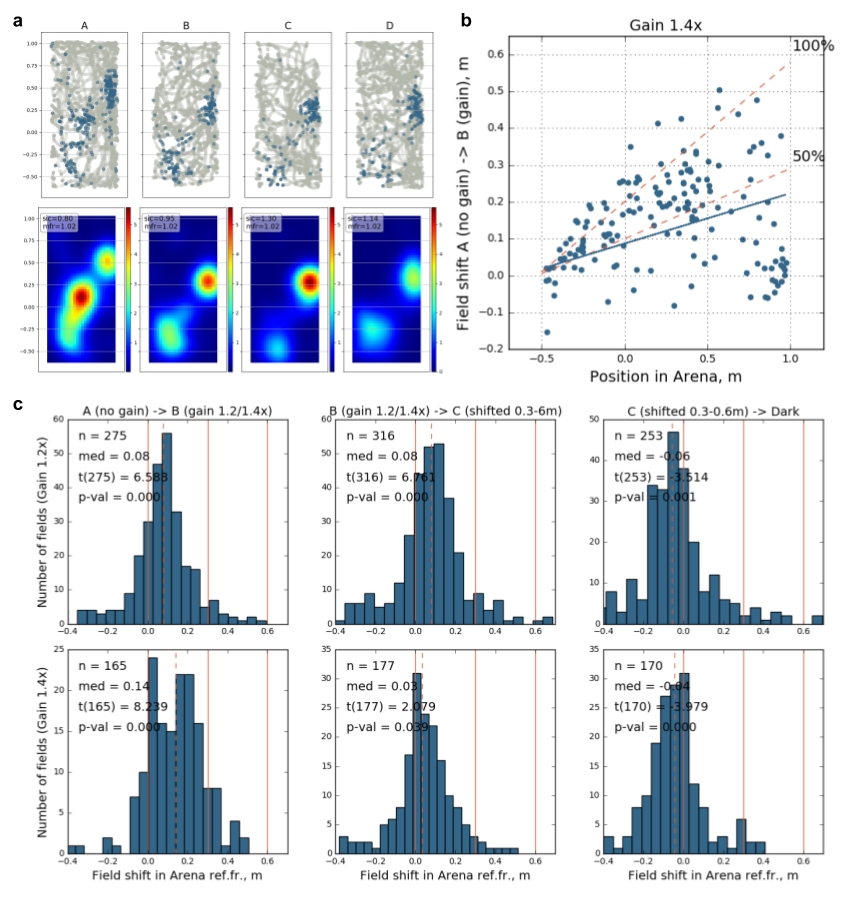
\includegraphics[width=150mm]{figures/F28_gain_14x.png}}
\caption[Sensory alternation in gradual mismatch in vGAIN 1.4x]{
vGAIN 1.4x and analysis of GAIN experiments. (a) An example place cell with a field active in all conditions. The gradual shift of the field along the shift of the visual reference frame (north -> south) shows influence of visual objects and cues. Note that in contrast to the gain 1.2x condition, a field is no longer influenced by vision when conflict is too large (B -> C). (b) Place field shifts between no-gain (A) and gain (B) conditions plotted against  the position in the arena. Dashed lines indicate the amount of conflict between visual and boundary-defined reference frames (100\% reflects the amount of conflict at the Y-axis). Note neurons encode the weighted average between two reference frames (blue linear regression bar), that linearly grows with the amount of conflict, until the conflict does not exceed ~0.4m. At larger conflicts > 0.4m there is a significant drop in the fraction of cells influenced by the visual reference frame. (c) Distribution of place field shifts for no gain (A) - gain (B) and gain (B) - no gain shifted (C) conditions shows continuous influence of the visual reference frame at smaller conflicts, similar to the vSHIFT experiment (top row, left and middle). A small shift back after the lights are off (top right plot) shows the overall recalibration of the spatial map between original and shifted conditions, similar to vSHIFT - visual. In contrast, the initial influence of the visual reference frame (bottom left) stops when the conflict becomes too large (bottom middle).
}
\label{fig:F28_gain_14x}
\end{figure}

A typical example of the place field shift is shown on Figure 28a. At first, a place field follows the visual projection and shifts in the direction of the conflict, encoding a weighted combination of the estimations (A -> B). However, after we asymmetrically reduce back the gain to no gain condition (B -> C) bringing two reference frames in a larger 0.6m conflict relative to the original condition, the place field tends to ignore further visual shift and keeps its spatial preference relative to the arena boundaries. This ignorance of the visual but not self-motion, or path integration driven spatial preference is confirmed by the stable spatial in darkness after the shifted condition (C -> D).

In total, 165, 177 and 170 place fields from 2 animals were recorded in the vGAIN 1.4x experiment for each condition (no gain - gain - no gain shifted), respectively. On the population level, as expected from the multisensory integration, cells tend to follow the visual reference frame in a weighted combination manner (Figure 28b, left part of the plot) at arena south, where the conflict between reference frames is relatively small (0 - 0.3m). However, at an arena north where the conflict exceeds a certain threshold, there is a decrease in the concentration of place fields following the visual projection in favor of the self-motion, boundary-defined input (Figure 28b, right part of the plot). This would be in line with an assumption, that cells tend to abandon one of the inputs at larger sensory conflicts.

Similar to the vSHIFT - visual experiment, the distributions of the place cell shift for the vGAIN 1.2x show overall shift of 0.17m between original (A) and shifted (C) conditions (e.g. “shift via gain”, Figure 28c top left plots). Interestingly, that turning the lights off at the end of the session led to a significant, but relatively small shift back of the overall spatial representation (Figure 28c top right plot), but not to the original position, which again supports the hypothesis of the recalibration of the self-motion based spatial representation by inducing a visual conflict (see visual conflict induces recalibration of the self-motion based map). For the 1.4x gain, enabling gain with asymmetric conflict leads to an overall significant shift of 0.14m at the population level (Figure 28c bottom left plot), smaller that the average between estimations given two reference frames, probably because cells tend to ignore visual reference frame at larger conflicts at the northern part of the arena. Further conflict from gain to no gain shifted (B -> C) does not have any further influence on the place cell location (Figure 28c bottom middle plot), potentially because of an overall larger conflict between original and shifted conditions (A -> C, 0.6m). Similar to the gain 1.2x, a small shift back is detected after the lights are off (Figure 28c bottom right plot), contributing to the recalibration hypothesis.
